% common part for every lection

\documentclass{beamer}

\usetheme{Warsaw}
\usefonttheme[onlylarge]{structurebold}
\setbeamerfont*{frametitle}{size=\normalsize,series=\bfseries}
\setbeamertemplate{navigation symbols}{}

\usepackage{pdfpages}
\usepackage{soul}
\usepackage{ucs}
\usepackage[utf8x]{inputenc}
\usepackage[TS1,T2A]{fontenc}
\usepackage[english,russian]{babel}
\usepackage{times}
\usepackage{listings}

\author[Author, Vlad Shakhov]{Влад 'mend0za' Шахов\\Linux \& Embedded Team Leader}

\institute[SaM Solutions]
{
  Linux \& Embedded Department
}

\date[Dec 2012]

\subject{Linux QA training}

\pgfdeclareimage[height=1.5cm]{sam-solutions-logo}{clipart/sam-solutions-elinux}

\logo{\pgfuseimage{sam-solutions-logo}}

\graphicspath{{./clipart/}}



\title[SaM Solutions. Linux QA Training]
{
  Часть 3.\\
  Файловая система, введение
}

\begin{document}
\begin{frame}
  \titlepage
\end{frame}

\section{Общие сведения}
\begin{frame}{Определения}[fragile]
  \begin{itemize}
    \item В UNIX (и Linux) файлы организованы в виде \emph{единой древовидной структуры} (дерева), называемой \alert{файловой системой}.
    \item \alert{Каждый файл имеет имя}, определяющее его расположение в дереве FS.
    \item Корнем дерева является \alert{корневой каталог} (root directory), имеющий имя \alert{"/"}.
  \end{itemize} \pause

  \begin{itemize}
    \item \alert{полный путь} начинается с \alert{/}(корневого каталога), каталоги разделяются также \alert{/}. \newline
      Пример: /home/user/.ssh/authorized\_key
    \item \alert{относительный путь} - от текущего каталога \newline
      Примеры: ../user10/.bashrc; ./script; ls script
  \end{itemize}

\end{frame}

\begin{frame}{Дерево файловой системы - простое}
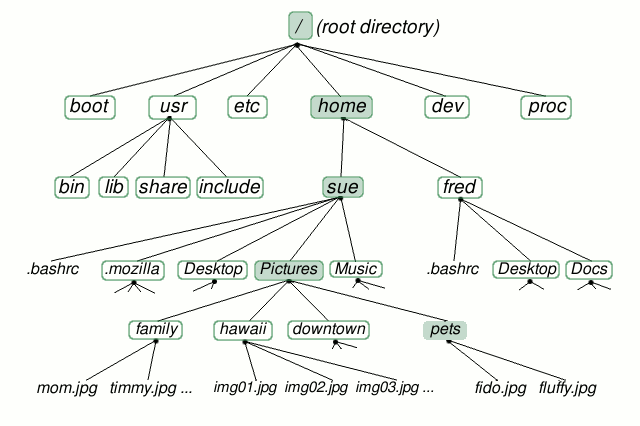
\includegraphics[height=8cm]{filesystem} 
\end{frame}

\begin{frame}{Дерево файловой системы - среднее}
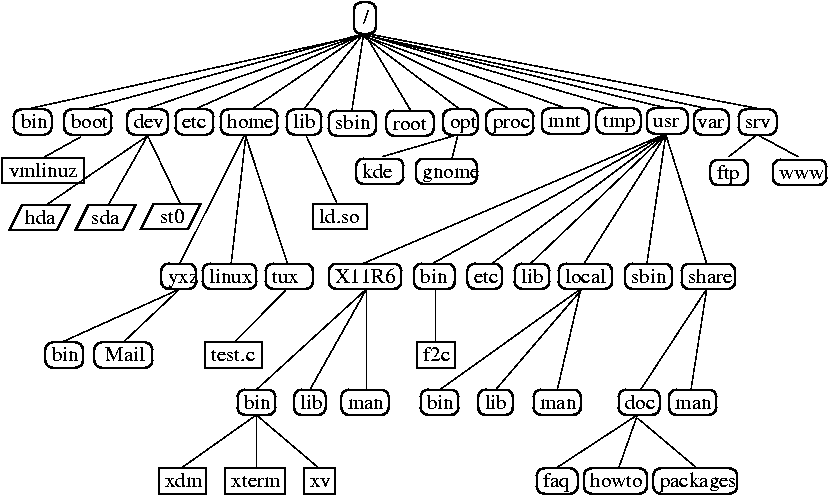
\includegraphics[height=7cm]{filesystem2} 
\end{frame}

\begin{frame}{Дерево файловой системы - сложное}
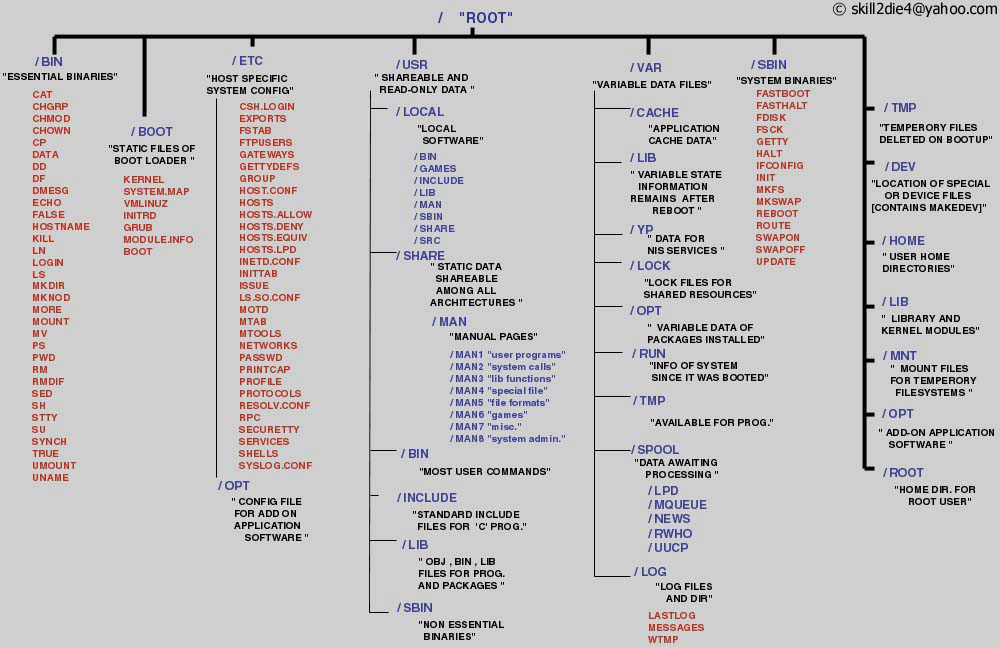
\includegraphics[height=7cm]{filesystem3} 
\end{frame}

\begin{frame}{Навигация}
\end{frame}

\end{document}
